\documentclass{article}
\usepackage[utf8]{inputenc}
\usepackage{graphicx}
\usepackage{amsmath, amsthm, amssymb}
\usepackage{multicol}
\usepackage{svg}
\usepackage{caption}
\usepackage{vmargin}
\usepackage[hidelinks]{hyperref}

\theoremstyle{definition}
\newtheorem{defi}{Definition}[section]
\newtheorem{theorem}{Theorem}[section]
\newtheorem{proposition}{Proposition}[section]
\newtheorem{lemma}{Lemma}[section]

\title{Constructions of $\mathbb{N}$, $\mathbb{Z}$, $\mathbb{Q}$, $\mathbb{R}$ and $\mathbb{C}$}
\author{Xiaozhe Yao\footnote{https://yaonotes.org/lecture-notes.html}}
\date{28 Oct 2019}
\begin{document}

\maketitle
\begin{center}
    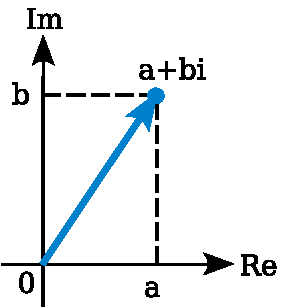
\includegraphics[width=60px]{Analysis/images/complex-number.pdf}
\end{center}

\section{Introduction}


\section{Construction of $\mathbb{N}$}

\noindent\textbf{Definition 1.1.1 (Informal Definition of $\mathbb{N}$):} A natural number is any element of the set:

$\mathbb{N} := \{0,1,2,3,4,...\}$.

which is the set of all the numbers created by starting with at $0$ and then counting forward indefinitely.

But there are some problems and questions: We do not have the concepts of Set right now, and How do we know we can keep counting indefinitely? Why it won't cycle back to $0$? Also why you can perform addition, multiplication, etc?

The latter question seems easy to answer, we can define exponentiation as repeated multiplication, multiplication as repeated additions, addition as repeated counting forward. It seems like how we learn to do addition in our 3 or 4 years old. But increments or counting forward is not reducible to any operations anymore.

In all, to define natural numbers, we need two fundamental concepts, the beginning (zero number) $0$ and the increment operation. Similar to computer languages, we could use $n++$ to denote the successor of n. For example, $3++ = 4, (3++)++ = 5$. With these, we have the following axioms.

\noindent\textbf{Axiom 1.1 (Axiom of 0):} 0 is a natural number.

\noindent\textbf{Axiom 1.2 (Axiom of Successor):} If n is a natural number, then n++ is also a natural number.

To make things simpler, we can use another notation.

\noindent\textbf{Definition 1.3 (Definition of numbers notation):} we define 1 to be the number $0++$, 2 to be the number $(0++)++$, etc. In other words, $1 := 0++, 2 := 1++$.

\noindent\textbf{Proposition 1.4 (Proposition of natural numbers):} 3 is a natural number.

\textit{Proof:} By axiom 1.1, 0 is a natural number. By axiom 1.2, 1 := 0++ is a natrual number. Again, 2:=1++ is a natural number. Again, 3:=2++ is a natural number. $\hfill\blacksquare$

It seems we have done. But considering the following system with 0,1,2, in which the incremental operations cycles, i.e. 1:=0++, 2:=1++, but 2++ equals to 0. It happens in our daily life, such as the number of weekdays (7++ = 1). Therefore, with only Axiom 1.1 and Axiom 1.2, we cannot guarantee the natural numbers won't cycle back to 0. We need another axiom.

\noindent\textbf{Axiom 1.3 (0 is not successor):} 0 is not the successor of any natural number. i.e. we have $ n++ \neq$ 0, for any natural number $n$.

\noindent\textbf{Proposition 1.5 (Proposition of 0 $\neq$ any other number):} 0 is not equal to 4.

\textit{Proof:} By definition, 4 = 3++, and 3 is a natural number (according to Axiom 1.1 and 1.2). According to Axiom 1.3, 3++ $\neq 0$ hence, $4 \neq 0$. $\hfill\blacksquare$

\section{Construction of $\mathbb{Z}$}

\section{Construction of $\mathbb{Q}$}

\section{Construction of $\mathbb{R}$}

\section{Construction of $\mathbb{C}$}

\section{References}

Tao, Terence. \textbf{Analysis}. Vol. 1. Hindustan Book Agency, 2006.

\end{document}